\documentclass{article}
\usepackage{graphicx}
\usepackage{amsmath}

\begin{document}
\title{Maths Assignment}
\author{Karyampudi Meghana Sai\\ EE23BTECH11031}
\maketitle

\section*{Problem Statement}
Write the first five terms of the sequence \(a_n = \frac{n(n^2+5)}{4}\).

\section*{Solution}


The relation between x(n) and u(n):
\begin{align}
 x(n) = \left(\frac{(n+1)^3+5(n+1)}{4}\right) u(n)
 \end{align}
 Given that the unit step function \(u(n)\) is:

\begin{align} 
u(n) = \begin{cases} 0 & \text{if } n < 0 \\ 1 & \text{if } n \geq 0 \end{cases}
 \end{align}
Its Z-transform becomes:

\begin{align}
U(z) &= \sum_{n=0}^{\infty} z^{-n} = 1 + z^{-1} + z^{-2} + z^{-3} + \dotsb  \\
U(z) &= \frac{1}{1- z^{-1}}
\end{align}
ROC for the z transform of u(n):\\
\text{ROC of} U(z):$\lvert z \rvert > 1$\\
The Z-transform of $nu(n)$ is given by:
\begin{align}
\mathcal{Z}\{nu(n)\} &= -\frac{1}{z^{-1}} \frac{d}{dz}[U(z)]\\
\mathcal{Z}\{nu(n)\} &= \frac{z^{-1}}{(1 - z^{-1})^2}
\end{align}
\text{ROC is} $\lvert z \rvert > 1$\\
The Z-transform of $n^2u(n)$ is given by:
\begin{align}
\mathcal{Z}\{n^2u(n)\} &= \frac{1}{z^{-1}} \frac{d}{dz}[U(z)] + \frac{1}{z^{-2}} \frac{d^2}{dz^2}[U(z)]\\
\mathcal{Z}\{n^2u(n)\} &= \frac{(z^{-1})(1+z^{-1})}{(1-z^{-1})^3}
\end{align}
\text{ROC is} $\lvert z \rvert > 1$\\
The Z-transform of $n^3u(n)$ is given by:
\begin{align}
\mathcal{Z}\{n^3u(n)\} &= -\frac{1}{z^{-1}} \frac{d}{dz}[U(z)] - \frac{3}{z^{-2}} \frac{d^2}{dz^2}[U(z)] - \frac{1}{z^{-3}} \frac{d^3}{dz^3}[U(z)]\\
\mathcal{Z}\{n^3u(n)\} &= \frac{(z^{-1})(1+4z^{-1}+z^{-2})}{(1-z^{-1})^4}
\end{align}
\text{ROC is} $\lvert z \rvert > 1$\\
Now Z-transform of x(n) is given by:
\begin{align}
\mathcal{X}\{z\} &=\frac{\mathcal{Z}\{n^3u(n)\}}{4} +\frac{3\mathcal{Z}\{n^2u(n)\}}{4} +2\mathcal{Z}\{nu(n)\} +\frac{3\mathcal{Z}\{u(n)\}}{2}\\
\mathcal{X}\{z\} &=\frac{(z^{-1})(1+4z^{-1}+z^{-2})}{4(1-z^{-1})^4} +\frac{3(z^{-1})(1+z^{-1})}{4(1-z^{-1})^3} +\frac{2z^{-1}}{(1 - z^{-1})^2} +\frac{3}{2(1- z^{-1})}
\end{align}
\newpage


\begin{figure}
    \centering
    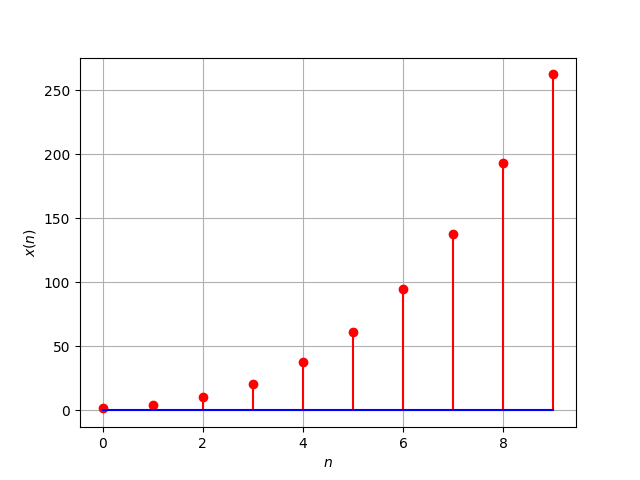
\includegraphics{plot.png}
    \caption{Plot of equation(1)}
    \label{fig:plot}
\end{figure}


\end{document}

